\section{Introduction}
Agriculture is one of the most fundamental resource of food production and also plays a vital role in keeping the economy running of every nation by contributing to the Gross Domestic Production. But there are several issues related to traditional methods of agriculture such as excessive wastage of water during field irrigation, dependency on non-renewable power source, time, money, human resource etc. Since every activity now a days is becoming smart, it needs to smartly develop agriculture sector for growth of country. Out project aims at developing a Smart Irrigation System using IoT Technology with the objective of automating the total job, providing adequate water required by crop by monitoring the moisture of soil and climate condition in order to prevent the wastage of water resources, resulting in many advantages for farmers. The irrigation at remote location from home will become easy and more comfortable. In addition, it will not only protect farmers from scorching heat and severe cold but also save their time otherwise required by the to-and-from journey to the field.

\subsection{Proposed Solution}
Modern agricultural methods propose an alternative way of water provisioning: instead of a daily/weekly irrigation, high-tech agricultural firms are moving towards slow, constant and lossless techniques that allow for water saving and a better quality of irrigation. In this optic, we decided to implement a smart system that is capable to compute real time the water need of the field and so to continuously adjust the water output that will be provisioned to plants. 
Of course, the success of this requires the water to be always available, but we all know that the seasons in which the need is higher are the ones with the lowest availability of natural water resources and vice versa: traditional irrigation methods tend to waste water abundance during wet periods and to overexploit aquifers during dry periods. 
In order to avoid that, the smart system makes use of a reservoir, i.e. a big container that collects water from the aquifer when the availability of it is much higher than the actual need, to be used as backup resource when aquifers are not enough. 
So, more precisely, the system uses provided sensors to determine the exact water output needed by plants; once this value has been computed, the system select from where to take the water and how to handle the reservoir, according to the water policy presented in the next indention. Finally it communicates output level and selected source to the tap actuator that handles the actual irrigation, and a new iteration will be performed very soon in order to guarantee the small but almost constant output.
WATER POLICY: if the aquifer flow is enough to cover needs, the source is the aquifer and the water excess is stored in the reservoir unless it is full. If it rains, no artificial irrigation is needed, so we turn-off the system in order to save energy and to allow the aquifer to grow again. If the aquifer is not enough to cover needs, the water will be entirely fetched from the reservoir, in order not to drain the aquifer; of course if the reservoir runs out of water the aquifer will be needed again. If the level detection system goes down, the water is taken from the aquifer.

\subsection{Deployment Structure}
The objective of this project is to adopt a smart irrigation system to water cultivated fields making use of the local water resources, such as aquifers and reservoirs, in the way of using the water resources as more eco-friendly as possible (e.g., without disrupting aquifers). Thus, we can consider two different locations to takes care: the \textbf{field} and the \textbf{water provisioning site},

For what concern the \textit{water provisioning site}, it is composed of sensors which have the mean of monitoring the water level both of the aquifers and reservoirs. In this way, the system and the user can know where to take water (by default the aquifer). Although, a single device for source may be enough, we decided to deploy multiple water level sensors in the same source in order to avoid errors in the monitoring (e.g., in the case of a single device if it is detected that the reservoir is empty, but it is not, the irrigation system will use the water from the aquifer pointlessly).
All water level sensors will make use of \textit{MQTT} as explained in the "MQTT Network" chapter.


The \textit{field site} is more articulated and will exploit multiple types of sensors and a single type of actuator. The actuator needed is the one capable of providing the water to the plants, which we called "tap actuator". This will be used in conjunction with the other sensors presents in the fields that will monitor the environment, specifically there will be temperature sensors, soil moisture sensors and a rain sensor. 
All these sensors and the tap actuator will exploit \textit{CoAP} as explained in the "CoAP Network" chapter.


\begin{figure}[H]
	\begin{subfigure}{\textwidth}
	\centering
		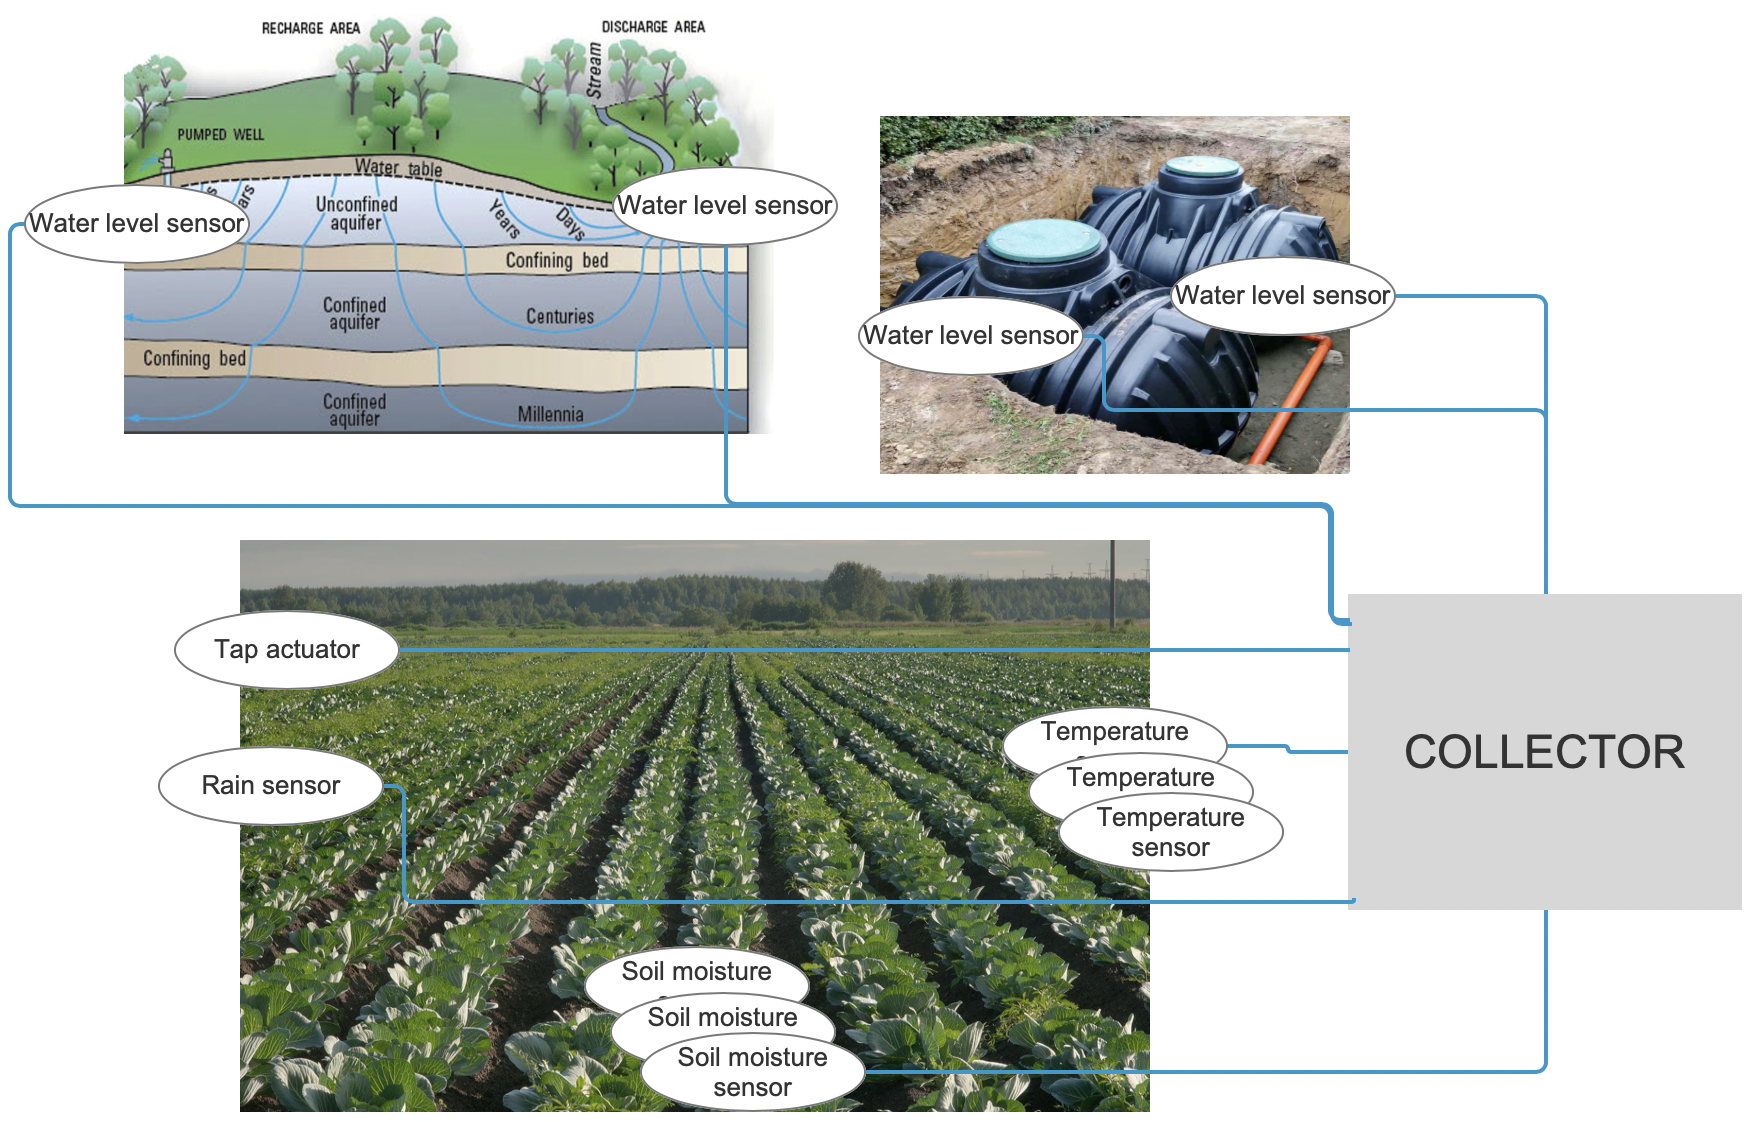
\includegraphics[width=1\linewidth]{img/deployment.png} 
	\end{subfigure}
\end{figure}